%% abtex2-modelo-trabalho-academico.tex, v-1.9.7 laurocesar
%% Copyright 2012-2018 by abnTeX2 group at http://www.abntex.net.br/ 
%%
% usando o modelo de trabalho acadêmico da ABNTex 2
\documentclass[
	% -- opções da classe memoir --
	12pt,				% tamanho da fonte
	openright,			% capítulos começam em pág ímpar (insere página vazia caso preciso)
	twoside,			% para impressão em recto e verso. Oposto a oneside
	a4paper,			% tamanho do papel. 
	% -- opções da classe abntex2 --
	%chapter=TITLE,		% títulos de capítulos convertidos em letras maiúsculas
	%section=TITLE,		% títulos de seções convertidos em letras maiúsculas
	%subsection=TITLE,	% títulos de subseções convertidos em letras maiúsculas
	%subsubsection=TITLE,% títulos de subsubseções convertidos em letras maiúsculas
	% -- opções do pacote babel --
	english,			% idioma adicional para hifenização
	french,				% idioma adicional para hifenização
	spanish,			% idioma adicional para hifenização
	brazil				% o último idioma é o principal do documento
	]{abntex2}

% ---
% Pacotes básicos 
% ---
\usepackage{lmodern}			% Usa a fonte Latin Modern			
\usepackage[T1]{fontenc}		% Selecao de codigos de fonte.
\usepackage[utf8]{inputenc}		% Codificacao do documento (conversão automática dos acentos)
\usepackage{indentfirst}		% Indenta o primeiro parágrafo de cada seção.
\usepackage{color}				% Controle das cores
\usepackage{graphicx}			% Inclusão de gráficos
\usepackage{microtype} 			% para melhorias de justificação
% ---
		
% ---
% Pacotes adicionais, usados apenas no âmbito do Modelo Canônico do abnteX2

% ---
% Pacotes de citações
% ---
\usepackage[brazilian,hyperpageref]{backref}	 % Paginas com as citações na bibl
\usepackage[alf]{abntex2cite}	% Citações padrão ABNT

% --- 
% CONFIGURAÇÕES DE PACOTES
% --- 

% ---
% Configurações do pacote backref
% Usado sem a opção hyperpageref de backref
\renewcommand{\backrefpagesname}{Citado na(s) página(s):~}
% Texto padrão antes do número das páginas
\renewcommand{\backref}{}
% Define os textos da citação
\renewcommand*{\backrefalt}[4]{
	\ifcase #1 %
		Nenhuma citação no texto.%
	\or
		Citado na página #2.%
	\else
		Citado #1 vezes nas páginas #2.%
	\fi}%
% ---

% ---
% Informações de dados para CAPA e FOLHA DE ROSTO
% ---
\titulo{Apostila de Netbeans para Novatos de Programação Java}
\autor{Paulino Ng}
\local{Brasil}
\data{2019, v-0.5.0}
%\orientador{}
%\coorientador{}
\instituicao{%
  Pang Co.
  \par
  Treinamento de Computação}
\tipotrabalho{Apostila}

\preambulo{Esta apostila visa mostrar aos novatos em programação como usar o Netbeans da Oracle como ambiente de desenvolvimento para programação Java.}

% ---
% Configurações de aparência do PDF final

% alterando o aspecto da cor azul
\definecolor{blue}{RGB}{41,5,195}

% informações do PDF
\makeatletter
\hypersetup{
     	%pagebackref=true,
		pdftitle={\@title}, 
		pdfauthor={\@author},
    	pdfsubject={\imprimirpreambulo},
	    pdfcreator={LaTeX with abnTeX2},
		pdfkeywords={abnt}{latex}{abntex}{abntex2}{trabalho acadêmico}, 
		colorlinks=true,       		% false: boxed links; true: colored links
    	linkcolor=blue,          	% color of internal links
    	citecolor=blue,        		% color of links to bibliography
    	filecolor=magenta,      		% color of file links
		urlcolor=blue,
		bookmarksdepth=4
}
\makeatother
% --- 

% ---
% Posiciona figuras e tabelas no topo da página quando adicionadas sozinhas
% em um página em branco. Ver https://github.com/abntex/abntex2/issues/170
\makeatletter
\setlength{\@fptop}{5pt} % Set distance from top of page to first float
\makeatother
% ---

% ---
% Possibilita criação de Quadros e Lista de quadros.
%
\newcommand{\quadroname}{Quadro}
\newcommand{\listofquadrosname}{Lista de quadros}

\newfloat[chapter]{quadro}{loq}{\quadroname}
\newlistof{listofquadros}{loq}{\listofquadrosname}
\newlistentry{quadro}{loq}{0}

% configurações para atender às regras da ABNT
\setfloatadjustment{quadro}{\centering}
\counterwithout{quadro}{chapter}
\renewcommand{\cftquadroname}{\quadroname\space} 
\renewcommand*{\cftquadroaftersnum}{\hfill--\hfill}

\setfloatlocations{quadro}{hbtp} % Ver https://github.com/abntex/abntex2/issues/176
% ---

% --- 
% Espaçamentos entre linhas e parágrafos 
% --- 

% O tamanho do parágrafo é dado por:
\setlength{\parindent}{1.3cm}

% Controle do espaçamento entre um parágrafo e outro:
\setlength{\parskip}{0.2cm}  % tente também \onelineskip

% ---
% compila o indice
% ---
\makeindex
% ---

% ----
% Início do documento
% ----
\begin{document}

% Seleciona o idioma do documento (conforme pacotes do babel)
\selectlanguage{brazil}

% Retira espaço extra obsoleto entre as frases.
\frenchspacing 

% ----------------------------------------------------------
% ELEMENTOS PRÉ-TEXTUAIS
% ----------------------------------------------------------
% \pretextual

% ---
% Capa
% ---
\imprimircapa
% ---

% ---
% Folha de rosto
% (o * indica que haverá a ficha bibliográfica)
% ---
\imprimirfolhaderosto*
% ---

% ---
% Inserir a ficha bibliografica
% ---

% Isto é um exemplo de Ficha Catalográfica, ou ``Dados internacionais de
% catalogação-na-publicação''. Você pode utilizar este modelo como referência. 
% Porém, provavelmente a biblioteca da sua universidade lhe fornecerá um PDF
% com a ficha catalográfica definitiva após a defesa do trabalho. Quando estiver
% com o documento, salve-o como PDF no diretório do seu projeto e substitua todo
% o conteúdo de implementação deste arquivo pelo comando abaixo:
%
% \begin{fichacatalografica}
%     \includepdf{fig_ficha_catalografica.pdf}
% \end{fichacatalografica}

\begin{fichacatalografica}
	\sffamily
	\vspace*{\fill}					% Posição vertical
	\begin{center}					% Minipage Centralizado
	\fbox{\begin{minipage}[c][8cm]{13.5cm}		% Largura
	\small
	\imprimirautor
	%Sobrenome, Nome do autor
	
	\hspace{0.5cm} \imprimirtitulo  / \imprimirautor. --
	\imprimirlocal, \imprimirdata-
	
	\hspace{0.5cm} \thelastpage p. : il. (algumas color.) ; 30 cm.\\
	
%	\hspace{0.5cm} \imprimirorientadorRotulo~\imprimirorientador\\
	
	\hspace{0.5cm}
	\parbox[t]{\textwidth}{\imprimirtipotrabalho~--~\imprimirinstituicao,
	\imprimirdata.}\\
	
	\hspace{0.5cm}
		1. Netbeans.
		2. Programação.
		2. Java.
		I. Pang Co.
		II. Apostila Netbeans 			
	\end{minipage}}
	\end{center}
\end{fichacatalografica}
% ---

% ---
% Dedicatória
% ---
\begin{dedicatoria}
   \vspace*{\fill}
   \centering
   \noindent
   \textit{ Este trabalho é dedicado aos que acreditam que é divertido resolver problemas com programação.} \vspace*{\fill}
\end{dedicatoria}
% ---

% ---
% Agradecimentos
% ---
\begin{agradecimentos}

Agradeço meus alunos de hoje, de ontem e de amanhã.

\end{agradecimentos}
% ---

% ---
% Epígrafe
% ---
\begin{epigrafe}
    \vspace*{\fill}
	\begin{flushright}
		\textit{``Don\'t Panic!\\
		Don\'t PANIC! \\
		DON\'T PANIC! \\
		(The Hitchhiker\'s Guide to the Galaxy, Douglas Adams)}
	\end{flushright}
\end{epigrafe}
% ---

% ---
% RESUMOS
% ---

% resumo em português
\setlength{\absparsep}{18pt} % ajusta o espaçamento dos parágrafos do resumo
\begin{resumo}
Esta apostila mostra rapidamente como começar a programar na linguagem Java com o uso do netbeans, a IDE (ambiente de desenvolvimento integrado) da Oracle.

 \textbf{Palavras-chave}: Netbeans. Java. Programação. IDE.
\end{resumo}

% resumo em inglês
\begin{resumo}[Abstract]
 \begin{otherlanguage*}{english}
   This booklet summarizes Oracle's tutorial on using netbeans, the IDE (integrated development environment) for Java programming.

   \vspace{\onelineskip}
 
   \noindent 
   \textbf{Keywords}: Netbeans. Java. Programming. IDE.
 \end{otherlanguage*}
\end{resumo}

% resumo em francês 
\begin{resumo}[Résumé]
 \begin{otherlanguage*}{french}
    Cette brochure résume le tutorial d’Oracle sur l’utilisation de netbeans, l’environnement de développement intégré (IDE) pour la programmation Java.
 
   \textbf{Mots-clés}: Netbeans. Java. Programação. IDE.
 \end{otherlanguage*}
\end{resumo}
% ---

% ---
% inserir lista de ilustrações
% ---
\pdfbookmark[0]{\listfigurename}{lof}
\listoffigures*
\cleardoublepage
% ---

% ---
% inserir lista de quadros
% ---
\pdfbookmark[0]{\listofquadrosname}{loq}
\listofquadros*
\cleardoublepage
% ---

% ---
% inserir lista de tabelas
% ---
\pdfbookmark[0]{\listtablename}{lot}
\listoftables*
\cleardoublepage
% ---

% ---
% inserir lista de abreviaturas e siglas
% ---
\begin{siglas}
  \item[IDE] Integrated Development Environment
  \item[JDK] Java Development Kit
  \item[JRE] Java Realtime Environment
  \item[SE] Standard Edition
  \item[EE] Enterprise Edition
  \item[ME] Mobile Edition
\end{siglas}
% ---

% ---
% inserir lista de símbolos
% ---
%\begin{simbolos}
%  \item[$ \Gamma $] Letra grega Gama
%  \item[$ \Lambda $] Lambda
%  \item[$ \zeta $] Letra grega minúscula zeta
%  \item[$ \in $] Pertence
%\end{simbolos}
% ---

% ---
% inserir o sumario
% ---
\pdfbookmark[0]{\contentsname}{toc}
\tableofcontents*
\cleardoublepage
% ---



% ----------------------------------------------------------
% ELEMENTOS TEXTUAIS
% ----------------------------------------------------------
\textual

% ----------------------------------------------------------
% Introdução (exemplo de capítulo sem numeração, mas presente no Sumário)
% ----------------------------------------------------------
\chapter{Introdução}
% ----------------------------------------------------------

A maioria dos estudantes de cursos superiores da área de computação do Brasil, a partir dos anos 2000 aprende na faculdade a programar em Java. Na proposta inicial da linguagem, o Java era uma linguagem orientada a objetos relativamente simples - Java 1.0.
% Com o passar do tempo, alguns dos seus princípios de base foram sendo esquecidos - inexistência de conversão automática de tipos, ... Hoje, perto do final da segunda década do século XXI, o Java se tornou extremamente complexo. Da biblioteca inicial de menos de 1000 classes, hoje o JDK-SE é distribuído com quase um milhão de classes.

No prólogo do livro \cite{livro-bluej}, o chefe do projeto inicial do Java, fala da dificuldade da filha para aprender a linguagem e o que ele percebe é que a dificuldade não é só com o Java, mas com a IDE usada no seu curso. Uma IDE, ambiente integrado de desenvolvimento, é um software bastante complexo que integra diversos outros programas/ferramentas. Às vezes, perde-se mais tempo aprendendo a usar corretamente uma IDE do que com a programação. Esta apostila pretende ensinar os primeiros passos da programação Java com a IDE Netbeans da Oracle.

Para comparar o uso ou não da IDE, o primeiro programa será mostrado sem o recurso da IDE. Posteriormente, usa-se-á a IDE para mostrar como ela pode ser útil para programações mais avançadas.

% ----------------------------------------------------------
% PARTE
% ----------------------------------------------------------
\part{Instalação dos softwares necessários}
% ----------------------------------------------------------

\chapter{Instalação do JDK}

Para poder programar em Java, o computador do aluno precisa ter instalado o JDK-SE, Java Development Kit - Standard Edition. O JDK inclui o programa compilador (javac), a biblioteca padrão chamada de Edição Padrão (SE - Standard Edition), esta é a biblioteca para desenvolvimento de aplicações para computadores de mesa, desktops, e computadores portáveis, laptops e notebooks. As outras bibliotecas são a EE, Enterprise Edition, para o desenvolvimento de aplicações para empresas e a ME, Mobile Edition, para o desenvolvimento de aplicações para dispositivos móveis. O JDK inclui também a JRE, Java Runtime Environment, que seu computador já deve ter para rodar aplicações Java, como o programa da receita federal. É importante que a JRE seja compatível com o compilador e as outras bibliotecas.

No momento da escrita desta apostila, existem diversos JDK SE, versões que vão da 6 a 11. Como uma extensão da disciplina, vai levar ao uso do Java EE, a versão mais avançada do Java EE é a 8. Assim, será exemplificado a seguir a instalação do JDK 8. Que pode ser baixado de:
https://www.oracle.com/technetwork/java/javase/downloads/jdk8-downloads-2133151.html.

\begin{figure}[h]
\begin{center}
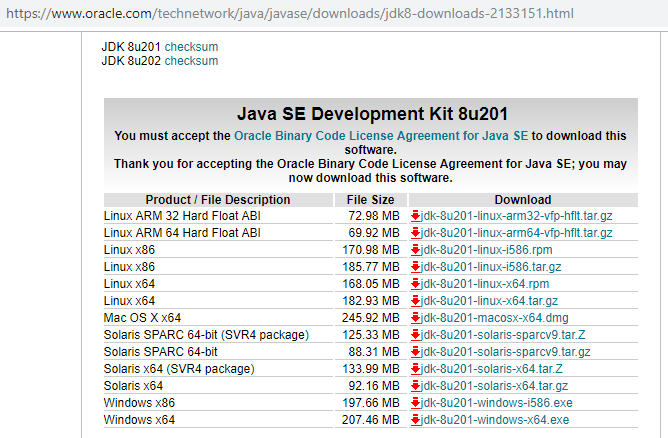
\includegraphics[scale=0.5]{jdk-download.png} 
\caption{Página para baixar o JDK SE}
\legend{Fonte: Snapshot do autor}
\label{fig:jdk-download}
\end{center}
\end{figure}

Baixe o arquivo adequado para o seu sistema, a figura \ref{fig:jdk-download} ilustra a página de download. Observe que para a instalação do JDK, é necessário usar o usuário com direitos administrativos do seu computador. Nesta apostila, as imagens mostram a execução dos programas dentro de um MS Windows 10, em língua inglesa. A instalação do JDK passa por duas etapas: na primeira é instalado o JDK e na segunda é instalado o JRE.

Um problema com o instalador no MS Windows é sua insistência em instalar os programas no diretório:
\begin{verbatim}
C:\Program Files\Java
\end{verbatim}

Em português, o diretório é o \texttt{C:$\backslash$Arquivo De Programas$\backslash$Java}. Ambos os nomes de diretórios possuem espaços no nome. Isto provoca problemas desnecessários para programas que usam o JDK e o JRE. Para evitar esta situação, na instalação, faça os programas serem instalados num diretório tal que não haja espaço no nome dos diretórios. Por exemplo, a figura \ref{jdk-dirs} mostra que a instalação foi feita nos diretórios C:$\backslash$User$\backslash$Public$\backslash$Java$\backslash$jdk8-201 e C:$\backslash$User$\backslash$Public$\backslash$Java$\backslash$jre8-201.

\begin{figure}[h]
\begin{center}
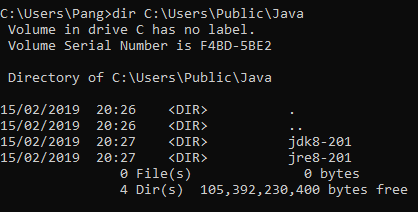
\includegraphics[scale=0.5]{jdk-dirs.png} 
\caption{Localização da instalação da JDK e da JRE sem espaços nos nomes de diretórios}
\legend{Fonte: Snapshot do autor}
\label{jdk-dirs}
\end{center}
\end{figure}

A existência de espaços nos nomes provocam problemas principalmente com o \emph{Tomcat} e outros servidores que usam o Java. Para estes programas funcionarem, é necessário configurar uma variável de ambiente, a JAVA\_HOME que deve dar o diretório de base do JDK.

A figura \ref{sys-var} mostra o acesso à configuração das variáveis de sistema. Para chegar a estas telas, acionar as teclas janela+pause (aperte simultaneamente na tecla windows e na tecla pause) dá acesso ao painel de controle do Sistema, selecione o \texttt{Ajuste de Sistema Avançado} e você terá a tela da figura \ref{sys-var}. Crie uma \textbf{Nova} variável de sistema com o nome \texttt{JAVA\_HOME}. No valor a ser atribuído à variável, coloque o diretório onde foi instalado o JDK. Para completar, configure a variável PATH. Selecione-a e clique em \texttt{Editar}. Na tela de edição, acrescente:

\begin{verbatim}
%JAVA_HOME%\bin
\end{verbatim}

\begin{figure}[h]
\begin{center}
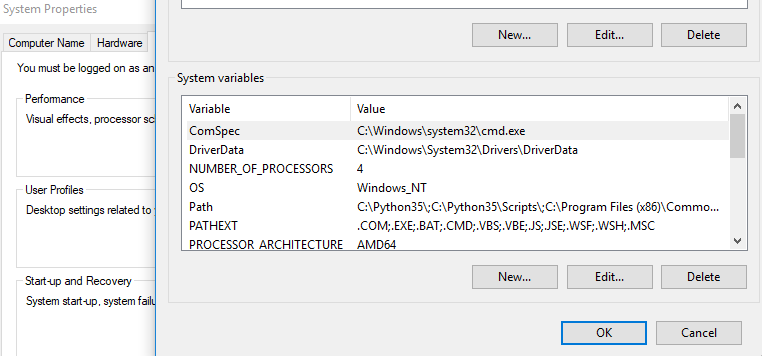
\includegraphics[scale=0.5]{sys-var.png} 
\caption{Configuração das variáveis de sistema no MS Windows}
\legend{Fonte: Snapshot do autor}
\label{sys-var}
\end{center}
\end{figure}

Dê \texttt{OK} para as mudanças. Feche as janela de \texttt{Prompt do DOS} e abra uma nova. Você dever capaz agora de acionar o compilador na linha de comando como mostrado na figura \ref{test-vars}.

\begin{figure}[h]
\begin{center}
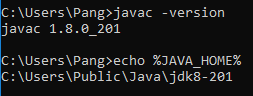
\includegraphics[scale=0.5]{test-vars.png} 
\caption{Acesso ao compilador Java e à variável JAVA\_HOME}
\legend{Fonte: Snapshot do autor}
\label{test-vars}
\end{center}
\end{figure}

% ----------------------------------------------------------
% PARTE
% ----------------------------------------------------------
\part{Escrita, compilação e execução dos primeiros programas}
% ----------------------------------------------------------



% ----------------------------------------------------------
% PARTE
% ----------------------------------------------------------
\part{Resultados}
% ----------------------------------------------------------

% ---
% primeiro capitulo de Resultados
% ---
\chapter{Lectus lobortis condimentum}
% ---

% ---
\section{Vestibulum ante ipsum primis in faucibus orci luctus et ultrices
posuere cubilia Curae}
% ---

% ----------------------------------------------------------
% Finaliza a parte no bookmark do PDF
% para que se inicie o bookmark na raiz
% e adiciona espaço de parte no Sumário
% ----------------------------------------------------------
\phantompart

% ---
% Conclusão
% ---
\chapter{Conclusão}
% ---

%\lipsum[31-33]

% ----------------------------------------------------------
% ELEMENTOS PÓS-TEXTUAIS
% ----------------------------------------------------------
\postextual
% ----------------------------------------------------------

% ----------------------------------------------------------
% Referências bibliográficas
% ----------------------------------------------------------
\bibliography{netbeans-references}

% ----------------------------------------------------------
% Glossário
% ----------------------------------------------------------
%
% Consulte o manual da classe abntex2 para orientações sobre o glossário.
%
%\glossary

% ----------------------------------------------------------
% Apêndices
% ----------------------------------------------------------

% ---
% Inicia os apêndices
% ---
\begin{apendicesenv}

% Imprime uma página indicando o início dos apêndices
\partapendices

% ----------------------------------------------------------
\chapter{Quisque libero justo}
% ----------------------------------------------------------

%\lipsum[50]

% ----------------------------------------------------------
\chapter{Nullam elementum urna vel imperdiet sodales elit ipsum pharetra ligula
ac pretium ante justo a nulla curabitur tristique arcu eu metus}
% ----------------------------------------------------------
%\lipsum[55-57]

\end{apendicesenv}
% ---


% ----------------------------------------------------------
% Anexos
% ----------------------------------------------------------

% ---
% Inicia os anexos
% ---
\begin{anexosenv}

% Imprime uma página indicando o início dos anexos
\partanexos

% ---
\chapter{Morbi ultrices rutrum lorem.}
% ---
%\lipsum[30]

% ---
\chapter{Cras non urna sed feugiat cum sociis natoque penatibus et magnis dis
parturient montes nascetur ridiculus mus}
% ---

%\lipsum[31]

% ---
\chapter{Fusce facilisis lacinia dui}
% ---

%\lipsum[32]

\end{anexosenv}

%---------------------------------------------------------------------
% INDICE REMISSIVO
%---------------------------------------------------------------------
\phantompart
\printindex
%---------------------------------------------------------------------

\end{document}
